% -*- latex -*-
%%%%%%%%%%%%%%%%%%%%%%%%%%%%%%%%%%%%%%%%%%%%%%%%%%%%%%%%%%%%%%%%
%%%%%%%%%%%%%%%%%%%%%%%%%%%%%%%%%%%%%%%%%%%%%%%%%%%%%%%%%%%%%%%%
%%%%
%%%% This text file is part of the source of
%%%% `Parallel Programming in MPI and OpenMP'
%%%% by Victor Eijkhout, copyright 2012-2025
%%%%
%%%% cuda.tex : cuda
%%%%
%%%%%%%%%%%%%%%%%%%%%%%%%%%%%%%%%%%%%%%%%%%%%%%%%%%%%%%%%%%%%%%%
%%%%%%%%%%%%%%%%%%%%%%%%%%%%%%%%%%%%%%%%%%%%%%%%%%%%%%%%%%%%%%%%

\Level 0 {Host and device}

Analogous to how OpenMP marked certain regions as parallel,
a \ac{CUDA} program marks certain function calls as
executable on a device.
\begin{itemize}
\item Host: the CPU where the execution starts
\item Device: one of possibly several attached \acp{GPU}.
\end{itemize}
Device code is recognizable by a keyword prefix,
either \indexcudashow{__global__} or \indexcudashow{__device__}.
The \indexcudashow{__host__} keyword marks host code, but that's the default.

\begin{lstlisting}
__global__ void some_cuda_function( /* parameters */ );
\end{lstlisting}
Device code needs have type \lstinline{void}:
return results have to be passed explicitly through memory.

\Level 1 {Hello world}

A device function that prints hello:
\cudaverbatimsnippet{cuhellodef}
And the main program launches this kernel on a grid of one block of size~1.
\cudaverbatimsnippet{cuhellouse}
We need the \indexcudashow{cudaDeviceSynchronize} function so that the host waits
until all device actions are completed.
\begin{figure}[ht]
  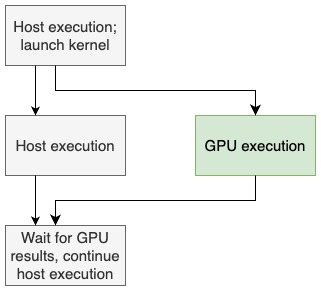
\includegraphics{hostgpuoverlap}
  \caption{Host and device activity}
  \label{fig:hostgpuoverlap}
\end{figure}
Normally, host and device actions can take place concurrently;
see figure~\ref{fig:hostgpuoverlap}.

The `triple chevron' syntax indicates how many block, and how many threads per block,
are used to launch the kernel.
You can put a 2D or 3D structure on the blocks by using the \indexcudashow{dim3}
coordinate structure:
\cudaverbatimsnippet{cuhello3use}
The coordinate of the block and the thread within the block can now be
found through the \indexcudashow{blockIdx} and \indexcudashow{threadIdx}
coordinate structures.

While the number of blocks can be large, the number of threads is limited.
The $x,y$ sides of the block cannot exceed~$1024$, and the $z$~side
can not exceed~$64$; the total size of the block is limited to~$1024$.

\Level 0 {Architecture}

You have seen the basic design of a grid of blocks,
where each block is a set of threads.
The blocks are distributed among the \acp{SM},
but even a single block can have more threads than
the \ac{SM} has cores, so
there is a further division in \indextermp{warp}.
A~warp is typically 32 threads.

\Level 1 {Thread indexing}

We need a way of identifying which CUDA thread executes a kernel.
Each kernel execution can query the (globally defined) variables
\indexcudadef{blockIdx} and \indexcudadef{threadIdx}.

It is possible to launch a kernel on more threads than
there are data points. In that case, your code could include
\begin{lstlisting}
int global_thread_id = blockIdx.x * blockDim.x + threadIdx.x; // or 2d, 3d variant
if ( global_thread_id > datasize ) return;
\end{lstlisting}

\Level 1 {Data transfer}

The host and device have separate memory, so you may need to
synchronize host data to the device.

\Level 2 {Explicit copy}

One strategy is allocate data separately for host and device.

Device memory is allocated with \indexcudashow{cudaMalloc}.
While the resulting pointer is visible to the host code,
the actual memory is on the device and you need to transfer data explicitly
between host and device with \indexcudadef{cudaMemcpy}.
This transfer can be between host and device in either direction,
or between two devices.

\begin{lstlisting}
cudaMemCpy( dest_ptr, orig_ptr, byte_size, direction );
// direction:
cudaMemcpyHostToDevice
cudaMemcpyDeviceToHost
cudaMemcpyDeviceToDevice
\end{lstlisting}

Example:
\cudaverbatimsnippet{cuhostdevalloc}

The data is then copied to the \ac{GPU}:
\cudaverbatimsnippet{cudatacopyin}
and after the kernel execution resulting data is copied back:
\cudaverbatimsnippet{cudatacopyout}

\Level 2 {Managed memory}

You can also allocate memory in a more abstract way:
`managed memory' can be written on the host,
but accessed from the device.
The actual mechanism that moves data back and forth
is based on \indexterm{paging}.
\cudaverbatimsnippet{cumanagedalloc}

\Level 1 {Shared memory}

\begin{figure}[ht]
  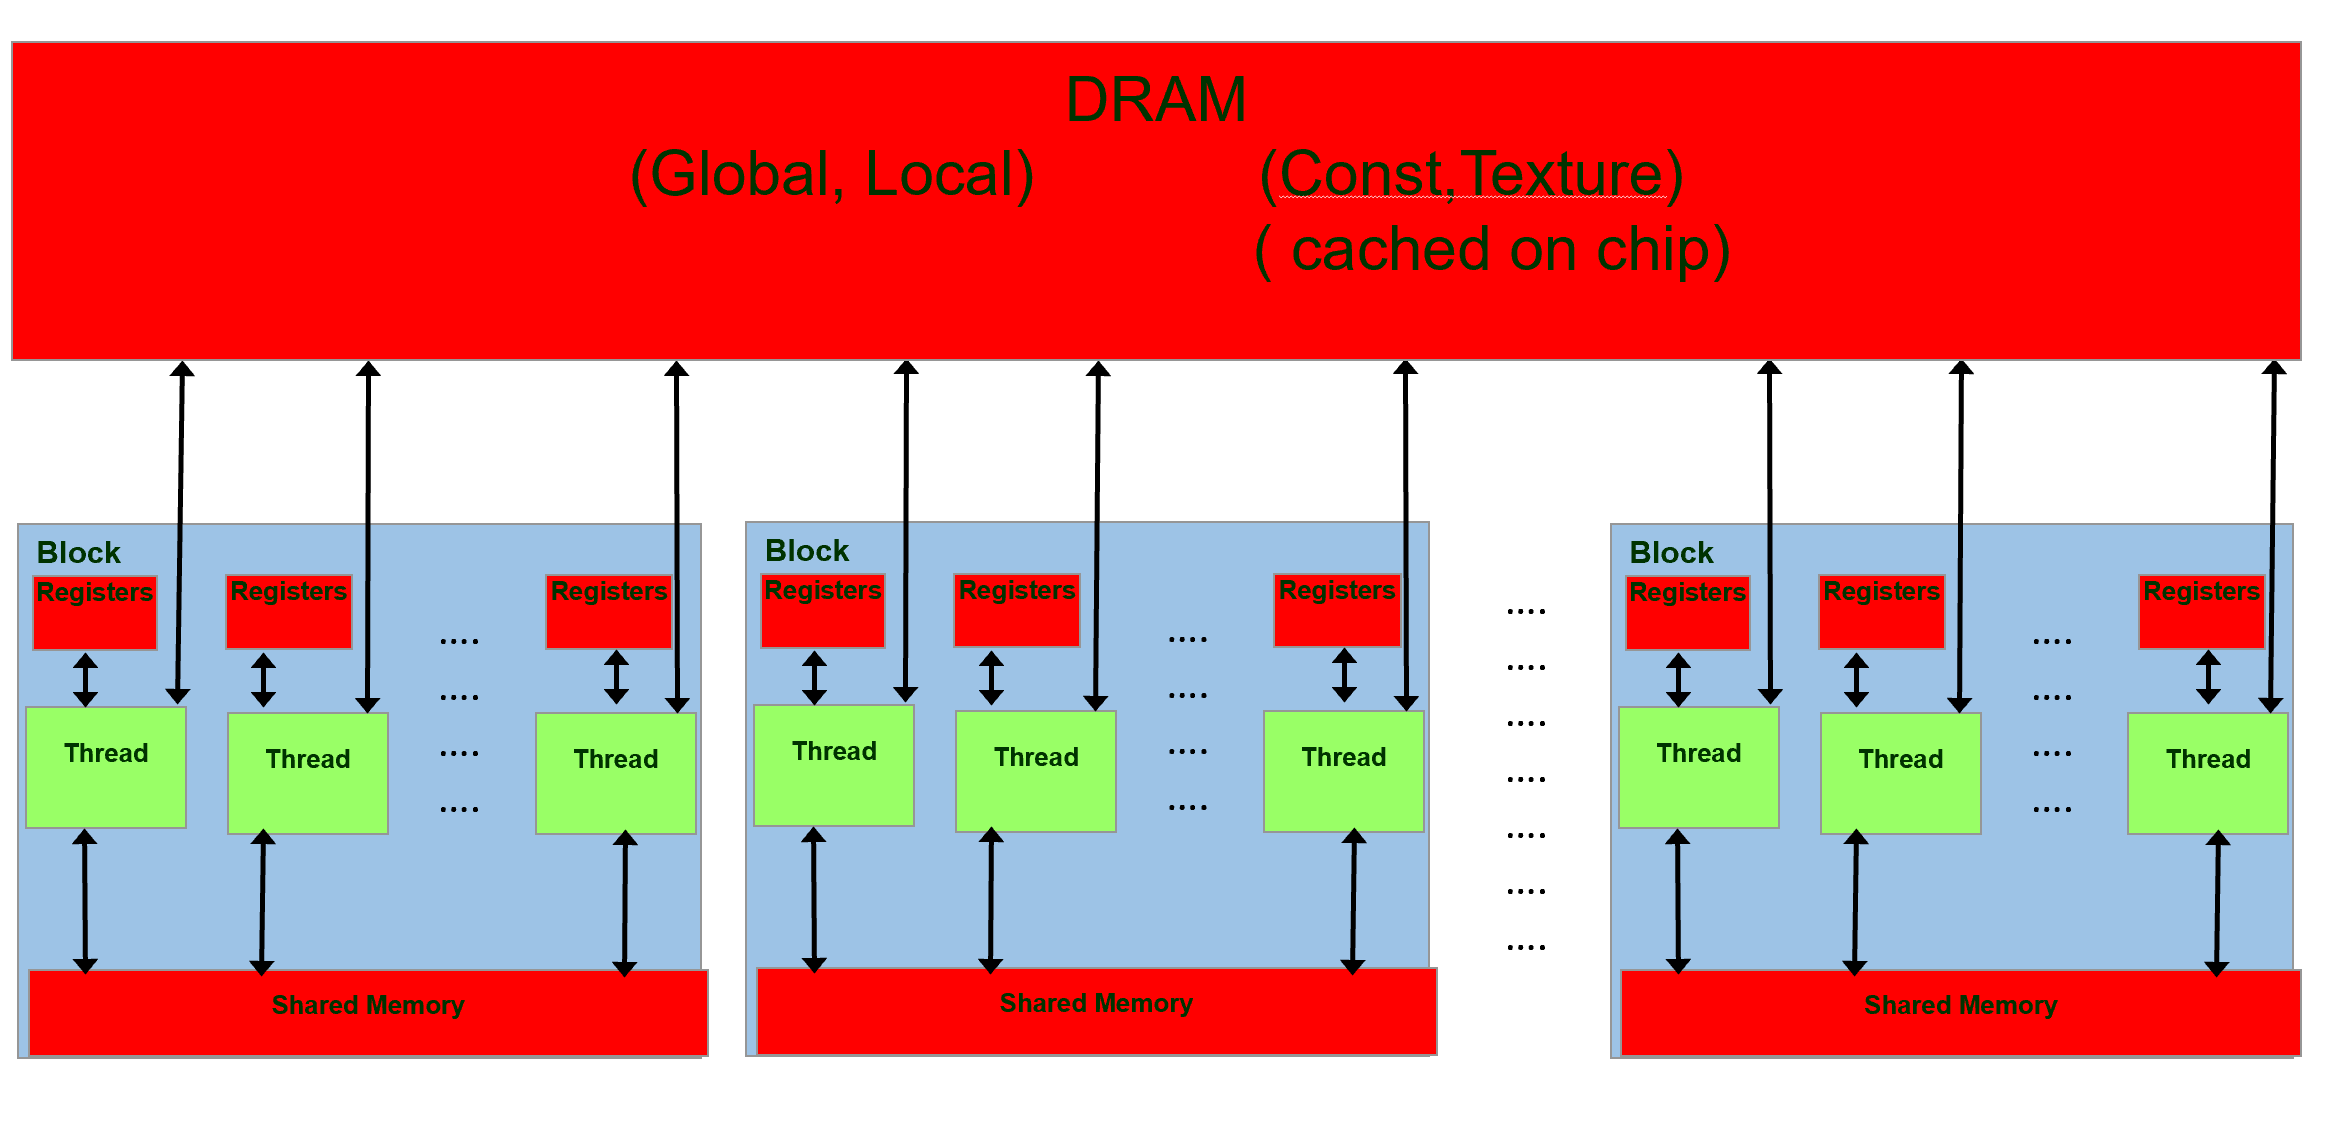
\includegraphics{nvidia-gpu-memory}  
  \caption{GPU memory structure}
  \label{fig:gpu-memory}
\end{figure}

The way we have coded so far, data is streamed from the
main memory of the \ac{GPU}.
For higher performance it is necessary to use the
\emph{shared memory}\index{memory!shared (GPU)}
of the threads in a block.
See figure~\ref{fig:gpu-memory}.

Shared memory is declared by adding the keyword
\indexcudashow{__shared__} to a regular array declaration:
\begin{lstlisting}
__shared__ float tmp[BLOCKSIZE];
\end{lstlisting}

\Level 0 {Querying}

Use \indexcudashow{cudaGetDeviceCount} to report how many \acp{GPU} are attached:
\cudaverbatimsnippet{cudevcount}
Possible errors: \indexcudashow{cudaErrorNoDevice} if there are no devices,
and \indexcudashow{cudaErrorInsufficientDriver} if the driver is too old.

Use \indexcudashow{cudaGetDeviceProperties}
to return a \indexcudashow{cudaDeviceProp} object:
\cudaverbatimsnippet{cudevprop}
Here are some of the properties:
\cudaverbatimsnippet{cudevprops}

\Level 0 {Synchronization}

\begin{itemize}
\item Threads in a warp are synchronized.
\item Threads in a thread block can be synchronized
  with the \indexcudadef{__syncthreads} function.
\item Thread blocks can not be synchronized.
\item Host and device can be synchronized
  with \indexcudashow{cudaDeviceSynchronize}.
\end{itemize}

\Level 1 {Reduction}

Fully data parallel operations are relatively easy
as we saw above.
When we start doing reductions we run into the fact that
thread blocks can not be synchronized.
That means that we call a \ac{CUDA} kernel to reduce
within each threadblock:
\cudaverbatimsnippet{cureductkernelproto}
but follow this up with a summation in the host code:
\cudaverbatimsnippet{cureductoutside}

\Level 1 {Implementation 1}

In the first implementation we let threads
at distances~$2,4,8,\ldots$ sum values
from offsets~$1,2,4,\ldots$:
\cudaverbatimsnippet{cureductkernel1}

The problem here is \indextermbus{warp}{divergence}:
different threads in a warp follow a different control path
through the conditional.

\Level 1 {Implementation 2}

We try to keep all threads in a warp active.
Instead of using threads at increasing strides
we use a contiguous block of threads.
\cudaverbatimsnippet{cureductkernel2}


\Level 0 {Performance}

The term \indextermbus{warp}{divergence} describes the situation
that the threads in a warp do not execute the same instruction.
\begin{lstlisting}
if ( threadIdx.x%2=0 )
  // do something
else
  // do something else
\end{lstlisting}
Since threads in a warp are tighly synchronized
this has a performance penalty.

\Level 1 {Profiling}

\indextermtt{ncu}
\url{https://docs.nvidia.com/nsight-compute/NsightComputeCli/index.html}

\begin{remark}
  Legacy: \indextermtt{nvprof}.
\begin{lstlisting}[language=bash]
nvprof --metrics branch_efficiency your_program
\end{lstlisting}
\end{remark}

\Level 0 {Other}
\Level 1 {Dynamic parallelism}

\ac{CUDA} routines can recursively call other
\ac{CUDA} routines.
The recursive call has a grid specification
as on the host.
\begin{lstlisting}
__global__
cuda_fn() {
  if (threadIdx.x%2==0)
    cuda_fn<<<1,blockDim.x/2>>>();
}
\end{lstlisting}

Compile flag: \lstinline[language=bash]{-rdc=true}.
